\documentclass{article}
% packages
\usepackage[margin=1 in]{geometry}
\usepackage{indentfirst}
\usepackage{titlesec}
\usepackage{enumitem}

%math package
\usepackage{amsmath}
\usepackage{mathtools}

% Use Links
\usepackage{xcolor}
\usepackage[colorlinks=true ,citecolor=blue, urlcolor=blue,urlbordercolor={1 0 0}]{hyperref} 


\title{HUDM 5126 Linear Models and Regression Analysis Homework 2\footnote{This homework is written in \LaTeX.}}
\author{Yifei Dong}
\date{Sep 9 2020}

\begin{document}
\maketitle
\section{Grade Point Average}
\indent 2.4 Refer to \textbf{Grade point average} Problem 1.19.

\begin{enumerate}[label=(\alph*)]
\item Obtain a 99 percent confidence interval for $\beta_{1}$. Interpret your confidence interval. Does it include zero? Why might the director of admissions be interested in whether the confidence interval includes zero?

The 99\% confidence interval for $\beta_{1}$ is (0.0054, 0.0723). We are 99\% confident that for each extra 1 point increase in ACT scores, student's Grade Point Average increase by as little as 0.0054 to as much as 0.0723. It does not include zero. The director of admissions should be interested in whether the confidence interval includes zero because if the confidence interval includes zero, then we should conclude that increase student's ACT scores have no contributions on GPA increase.

\item Test, using the test statistic \emph{t*}, whether or nor a linear association exists between student's ACT score (\emph{X}) and GPA at the end of the freshman year (\emph{Y}). Use a level of significance of .01. State the alternatives, decision rule, and conclusion.

\begin{center}
$H_{0}$: $\beta_{1}=0$

$H_{a}$: $\beta_{1} \neq 0$
\end{center}

The decision rule (Two-sided Test): 

\begin{center}
If $|t^*| \leq t(1-\alpha/2; n-2)$, conclude $H_{0}$

if $|t^*|> t(1-\alpha/2; n-2)$, conclude $H_{a}$
\end{center}

Since t-statistic=3.040 $>$ t(0.995,118)=2.618, we reject $H_{0}$ and conclude that $\beta_{1}$ is significant and not equal to 0.

\item What is the P-value of your test in part (b)? How does it support the conclusion reached in part (b)?

The P-value is 0.00292. Since 0.00292 $<$ 0.01, it supports the conclusion reached in part (b).

\end{enumerate}

\textbf{Extra Exercises\footnote{The graph is made using ggplot2 package. }}: The scatter plot with the regression line, confidence intervals and prediction intervals can be found in Figure~\ref{fig:plot1}.

\clearpage
\begin{figure}[htbp]
\begin{center}
\caption{This is a scatter plot with the regression line, confidence intervals and prediction intervals}
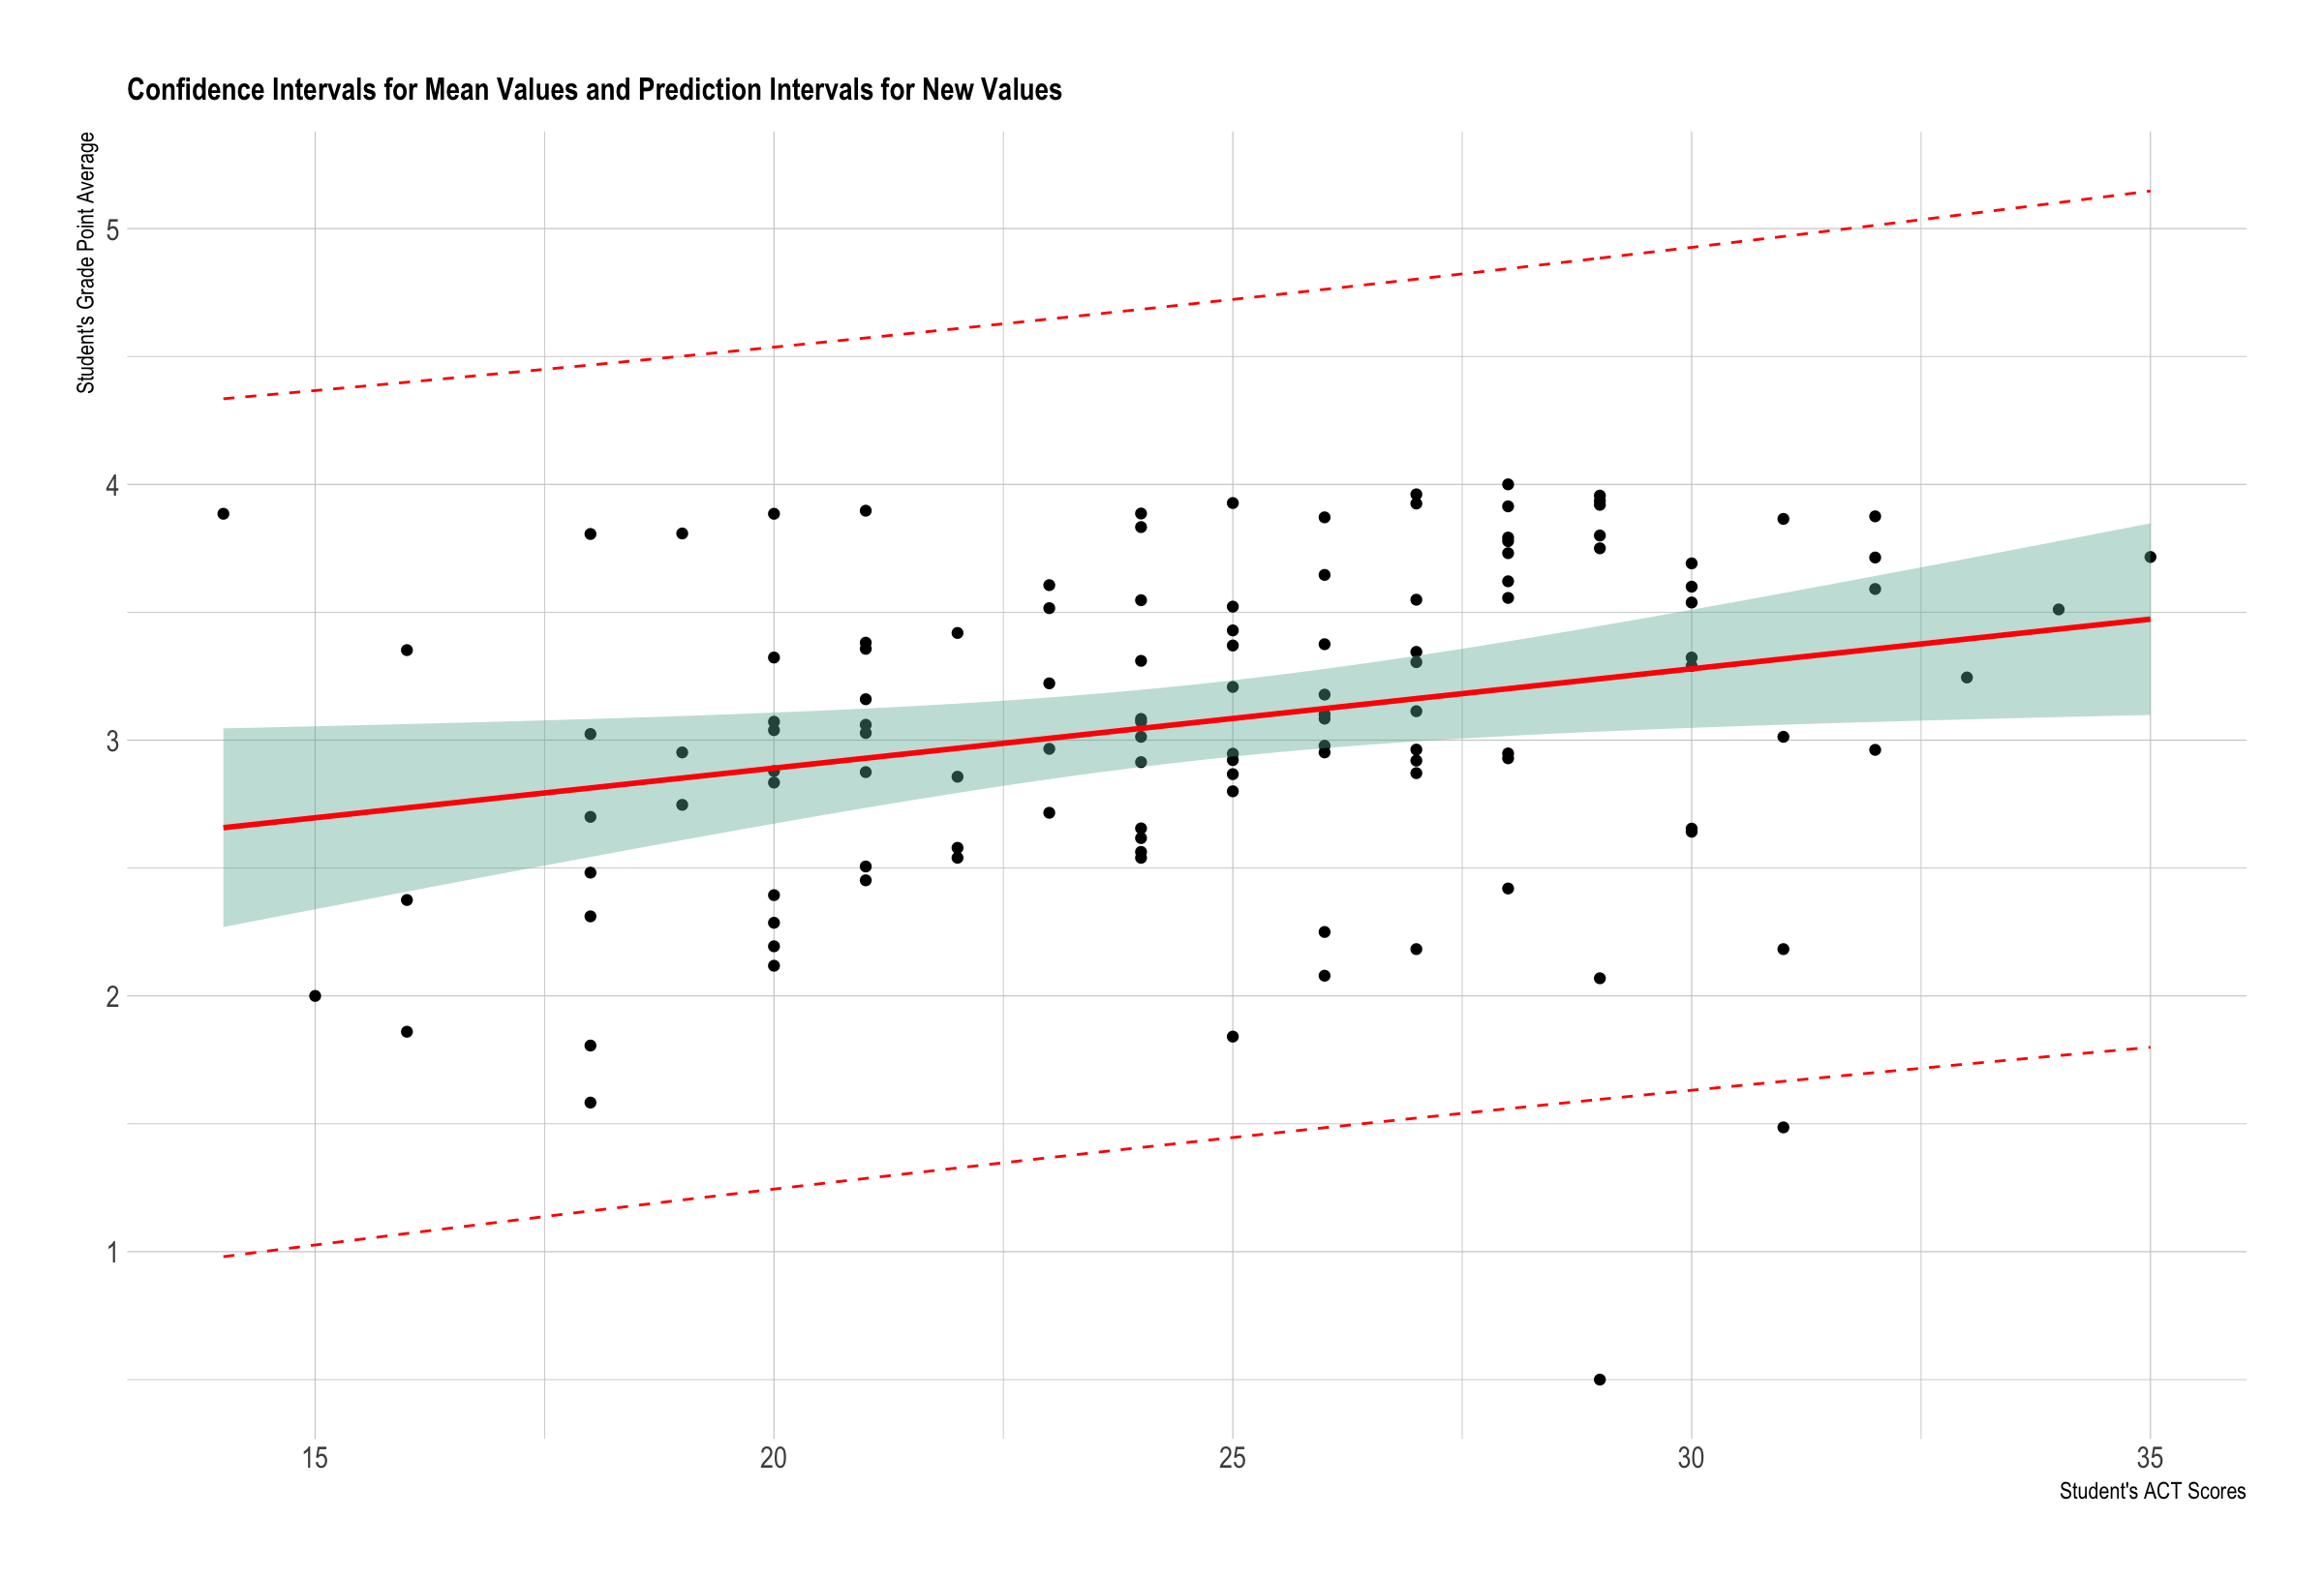
\includegraphics[width=150mm]{graph1.png}
\end{center}
\label{fig:plot1}
\end{figure}

\newpage
\section{Bid Preparation}
\indent 2.44 A building construction consultant studied the relationship between cost of bid preparation (\emph{$Y_{1}$}) and amount of bid (\emph{$Y_{2}$}) for the consulting firm's clients. In a sample of 103 bids prepared by clients, $r_{12}=.87$. Assume that bivariate normal model (2.74) applies.

\begin{enumerate}[label=(\alph*)]

\item Test whether or not $\rho_{12}=0$; control the risk of Type I error at .10. State the alternatives, decision rule, and conclusion. What would be the implication if $\rho_{12}=0$?
\begin{center}
$H_{0}$: $\rho_{12}=0$

$H_{a}$: $\rho_{12} \neq 0$
\end{center}

The decision rule: 

\begin{center}
If $|t^*| \leq t(1-\alpha/2; n-2)$, conclude $H_{0}$

if $|t^*|> t(1-\alpha/2; n-2)$, conclude $H_{a}$
\end{center}

\begin{equation}
t=\frac{r\sqrt{n-2}}{\sqrt{1-r^2}}=\frac{.87\cdot\sqrt{103-2}}{\sqrt{1-.87^2}}=17.73321
\end{equation}

t(.95,101)=1.66. Since 17.733 $>$ 1.66, we reject the null hypothesis and conclude that $\rho_{12} \neq 0$. If $\rho_{12}=0$, then we conclude that there is no linear association between cost of bid preparation (\emph{$Y_{1}$}) and amount of bid (\emph{$Y_{2}$}) for the consulting firm's clients. In the case where $Y_{1}$ and $Y_{2}$ are jointly normally distributed, $\rho_{12}=0$ implies that $Y_{1}$ and $Y_{2}$ are independent.

\item Obtain a 90 percent confidence interval for $\rho_{12}$. Interpret this interval estimate.

The point estimate of $\rho_{12}$ was $r_{12}$=.87. To obtain an approximate 90 percent confidence interval estimate, we require:

\begin{equation}
\mathbf{E}\{z'\}=\zeta=\frac{1}{2}\log_{e}(\frac{1+\rho_{12}}{1-\rho_{12}})=\frac{1}{2}\log_{e}(\frac{1+.87}{1-.87})=\frac{1}{2}\log_e(\frac{1.87}{.13})=1.3331
\end{equation}

\begin{equation}
\sigma^2\{z'\}=\frac{1}{n-3}=\frac{1}{103-3}=.01
\end{equation}

therefore, $\sigma=\sqrt{.01}=.1$. and $z(1-\alpha/2)=z(1-0.1/2)=z(1-.05)=z(.95)=1.645$.

Hence, the confidence limits for $\zeta$, are $1.333 \pm 1.645 (.1)$, and the approximate 90 percent confidence interval is:

\begin{center}
$1.1685 \leq \zeta \leq 1.4975$
\end{center}

To transform back to $\rho_{12}$, using the following equation,:

\begin{equation}
\rho_{12}=\frac{e^{2\zeta}-1}{1+e^{2\zeta}}
\end{equation}

We obtain:

\begin{center}
$0.824 \leq \rho_{12} \leq 0.905$
\end{center}

\item Convert the confidence interval in part(b) to a 90 percent confidence for $\rho^2_{12}$.

\begin{center}
$(0.824)^2 \leq \rho^2_{12} \leq (0.905)^2=0.679 \leq \rho^2_{12} \leq 0.819$
\end{center}


\end{enumerate}

\newpage
\section{Proof}
Show that the ratio SSR/SSTO is the same whether $Y_{1}$ is regressed on $Y_{2}$ or $Y_{2}$ is regressed on $Y_{1}$. [\emph{Hint}: Use (1.10a) and (2.51)].
\vspace{5mm}

Recall equation~\ref{eq:1.10a} and equation~\ref{eq:2.51}:
\begin{equation} \tag{1.10a}
b_{1}=\frac{\sum (X_{i}-\overline{X})(Y_{i}-\overline{Y})}{\sum(X_{i}-\overline{X})^2}
\label{eq:1.10a}
\end{equation}

\begin{equation} \tag{2.51}
SSR=b^2_{1}\sum (X_{i}-\overline{X})^2
\label{eq:2.51}
\end{equation}

First, $Y_{1}$ is regressed on $Y_{2}$, then $\widehat{Y_{1}}=b_{0}+b_{1}Y_{2}$

\begin{equation} \tag{3.11}
b_{1}=\frac{\sum (Y_{i2}-\overline{Y_{2}})(Y_{i1}-\overline{Y_{1}})}{\sum(Y_{i2}-\overline{Y_{2}})^2}
\end{equation}

\begin{equation} \tag{3.12}
SSR=\bigg[\frac{\sum (Y_{i2}-\overline{Y_{2}})(Y_{i1}-\overline{Y_{1}})}{\sum(Y_{i2}-\overline{Y_{2}})^2}\bigg]^2\big[\sum(Y_{i2}-\overline Y_{2})^2\big]
\end{equation}

\begin{equation} \tag{3.13}
SSTO=\sum(Y_{i1}-\overline{Y_{1}})^2
\end{equation}

therefore,

\begin{equation} \tag{3.14}
\frac{SSR(Y_{2})}{SSTO}=\frac{\big[\sum(Y_{i2}-\overline{Y_{2}})(Y_{i1}-\overline{Y_{1}})\big]^2}{\sum(Y_{i1}-\overline{Y_{1}})^2 \sum(Y_{i2}-\overline{Y_{2}})^2}
\label{eq:3.14}
\end{equation}

Second, $Y_{2}$ is regressed on $Y_{1}$, then $\widehat{Y_{2}}=b_{0}+b_{1}Y_{1}$

\begin{equation} \tag{3.21}
b_{1}=\frac{\sum (Y_{i1}-\overline{Y_{1}})(Y_{i2}-\overline{Y_{2}})}{\sum(Y_{i1}-\overline{Y_{1}})^2}
\end{equation}

\begin{equation} \tag{3.22}
SSR=\bigg[\frac{\sum (Y_{i1}-\overline{Y_{1}})(Y_{i2}-\overline{Y_{2}})}{\sum(Y_{i1}-\overline{Y_{1}})^2}\bigg]^2\big[\sum(Y_{i1}-\overline Y_{1})^2\big]
\end{equation}

\begin{equation} \tag{3.23}
SSTO=\sum(Y_{i2}-\overline{Y_{2}})^2
\end{equation}

therefore,

\begin{equation} \tag{3.24}
\frac{SSR(Y_{1})}{SSTO}=\frac{\big[\sum(Y_{i1}-\overline{Y_{1}})(Y_{i2}-\overline{Y_{2}})\big]^2}{\sum(Y_{i1}-\overline{Y_{1}})^2\sum(Y_{i2}-\overline{Y_{2}})^2}
\label{eq:3.24}
\end{equation}
\vspace{5mm}

Since equation~\ref{eq:3.14} equals equation~\ref{eq:3.24}, we conclude that the ratio SSR/SSTO is the same whether $Y_{1}$ is regressed on $Y_{2}$ or $Y_{2}$ is regressed on $Y_{1}$.

\end{document}